\documentclass{article}

\usepackage{graphicx}
\usepackage{tikz}
\usepackage{tikzsymbols}
\usetikzlibrary{calc,patterns,shapes.geometric}
\pagestyle{empty}
\usepackage[margin=0pt]{geometry}
\geometry{papersize={14in,12in}}

\def\centerarc[#1](#2)(#3:#4:#5){\draw[#1] ($(#2)+({#5*cos(#3)},{#5*sin(#3)})$) arc (#3:#4:#5);}

\begin{document}
	\begin{figure}
		\centering
		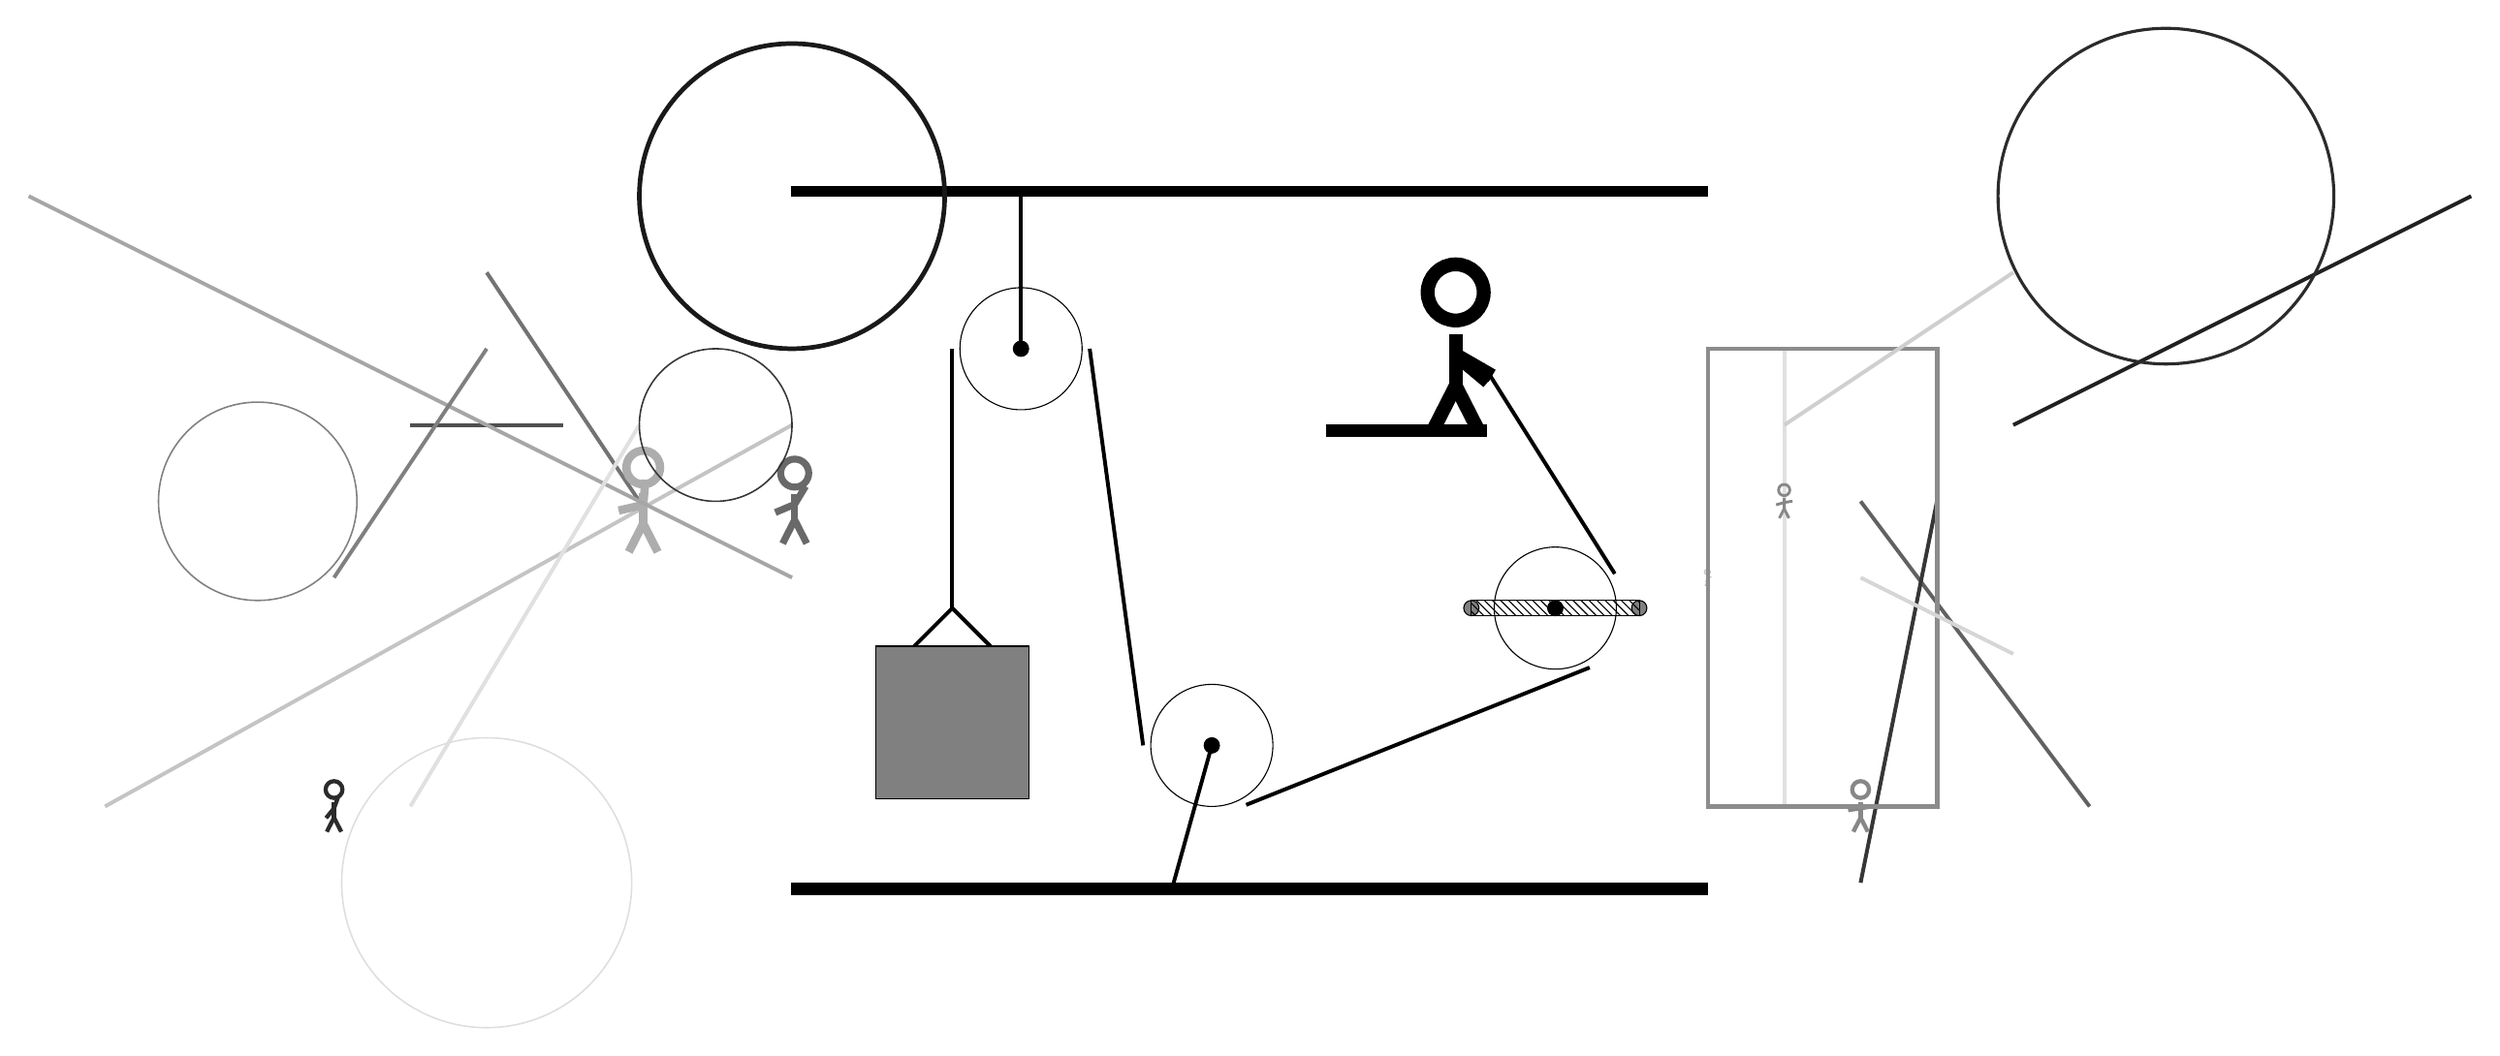
\begin{tikzpicture}
			%%%%% START %%%%%
			
			\draw[fill=black] (-2, 9) rectangle (10, 9.125);
			
			\draw (1, 7) circle (0.8);
			\draw[fill=black] (1, 7) circle (0.1);
			\draw[line width=0.5mm] (1, 9) -- (1, 7);
			
			\node[line width=0.3mm, color=black!23] at (10, 4) {\Strichmaxerl[1][65][21]};
			
			\draw[line width=0.5mm, color=black!12] (11, 7) rectangle (13, 1);
			\draw[line width=0.5mm, color=black!62](12, 5) -- (15, 1);
			\draw[line width=0.5mm, color=black!87](14, 6) -- (20, 9);
			\draw[line width=0.5mm, color=black!79](13, 5) -- (12, 0);
			\node[line width=0.4mm, color=black!47] at (12, 1) {\Strichmaxerl[3][9][9]};
			\draw[line width=0.6mm, color=black!45] (10, 7) rectangle (13, 1);
			
			\draw [line width=0.6mm, color=black!90](-2, 9) circle (2.0);
			\draw[line width=0.5mm, color=black!55](-6, 8) -- (-4, 5);
			\draw[line width=0.5mm, color=black!23](-2, 6) -- (-11, 1);
			
			\node[line width=0.7mm, color=black!59] at (-2, 5) {\Strichmaxerl[5][23][59]};
			\draw [line width=0.4mm, color=black!83](16, 9) circle (2.2);
			\node[line width=0.3mm, color=black!32] at (-4, 5) {\Strichmaxerl[6][13][85]};
			\draw[line width=0.5mm, color=black!69](-5, 6) -- (-7, 6);
			\draw[line width=0.5mm, color=black!16](12, 4) -- (14, 3);
			\draw[line width=0.5mm, color=black!35](-2, 4) -- (-12, 9);
			\draw [line width=0.2mm, color=black!50](-9, 5) circle (1.3);
			
			\draw[line width=0.5mm, color=black!19](14, 8) -- (11, 6);
			\draw[line width=0.5mm, color=black!12](-7, 1) -- (-4, 6);
			\node[line width=0.5mm, color=black!83] at (-8, 1) {\Strichmaxerl[3][51][70]};
			\draw [line width=0.2mm, color=black!13](-6, 0) circle (1.9);
			
			\node[line width=0.3mm, color=black!47] at (11, 5) {\Strichmaxerl[2][16][9]};
			\draw [line width=0.2mm, color=black!79](-3, 6) circle (1.0);
			\draw[line width=0.5mm, color=black!50](-6, 7) -- (-8, 4);
			
			\draw (3.5, 1.8) circle (0.8);
			\draw[fill=black] (3.5, 1.8) circle (0.1);
			\draw[line width=0.5mm] (3.5, 1.8) -- (3.0, 0);
			
			\draw[fill=white](8, 3.6) circle (0.8);
			\draw[fill=black] (8, 3.6) circle (0.1);
			\draw[fill=black!50] (9.1, 3.6) circle (0.1);
			\draw[fill=black!50] (6.9, 3.6) circle (0.1);
			\draw[pattern=north west lines, pattern color=black] (6.9, 3.7) rectangle (9.1, 3.5);
			
			\draw[line width=0.5mm](-0.4, 3.1) --  (0.1, 3.6) -- (0.6, 3.1);
			\draw[fill=black!50] (-0.9, 3.1) rectangle (1.1, 1.1);
			
			\draw[line width=0.5mm](0.1, 7) -- (0.1, 3.6);
			\centerarc[line width=0.5mm](1, 7)(180:0:0.9)
			\draw[line width=0.5mm](1.9, 7) -- (2.6, 1.8);
			\centerarc[line width=0.5mm](3.5, 1.8)(180:300:0.9);
			\draw[line width=0.5mm](3.95, 1.0206) -- (8.45, 2.8206);
			\centerarc[line width=0.5mm](8, 3.6)(300:390:0.9);
			\draw[line width=0.5mm](8.7794, 4.05) -- (7.05, 6.8);
			
			\node at (6.75, 7) {\Strichmaxerl[10][-220][-30]};
			\draw[fill=black] (5, 6) rectangle (7.1, 5.85);
			
			\draw[fill=black] (-2, 0) rectangle (10, -0.15);
			
			%%%%% END %%%%%
		\end{tikzpicture}
	\end{figure}	
\end{document}